\documentclass[tikz,border=8pt]{standalone}
% Shared look for every TikZ diagram. Load with % Shared look for every TikZ diagram. Load with % Shared look for every TikZ diagram. Load with \input{../../tools/tikz-style.tex}
\usepackage[T1]{fontenc}
\usepackage{lmodern}
\renewcommand{\sfdefault}{lmr}  % diagrams use the same serif as the text
\usetikzlibrary{arrows.meta, positioning, shapes.geometric, calc, fit, backgrounds}
\definecolor{cblue}{HTML}{4C78A8}
\definecolor{corange}{HTML}{F58518}
\definecolor{cgreen}{HTML}{54A24B}
\definecolor{cred}{HTML}{E45756}
\definecolor{cpurple}{HTML}{B279A2}
\definecolor{cgrey}{HTML}{6B6B6B}
\tikzset{
  every picture/.style={font=\sffamily, line width=1.2pt},
  box/.style={draw=#1, fill=#1!12, rounded corners=4pt, align=center, inner sep=7pt, minimum height=1.1cm},
  box/.default=cgrey,
  arrow/.style={-{Stealth[length=3mm]}, draw=cgrey, line width=1.4pt},
  title/.style={font=\sffamily\bfseries\Large},
  note/.style={font=\sffamily\small, text=cgrey, align=center},
}
\AtBeginDocument{\hyphenpenalty=10000 \exhyphenpenalty=10000}

\usepackage[T1]{fontenc}
\usepackage{lmodern}
\renewcommand{\sfdefault}{lmr}  % diagrams use the same serif as the text
\usetikzlibrary{arrows.meta, positioning, shapes.geometric, calc, fit, backgrounds}
\definecolor{cblue}{HTML}{4C78A8}
\definecolor{corange}{HTML}{F58518}
\definecolor{cgreen}{HTML}{54A24B}
\definecolor{cred}{HTML}{E45756}
\definecolor{cpurple}{HTML}{B279A2}
\definecolor{cgrey}{HTML}{6B6B6B}
\tikzset{
  every picture/.style={font=\sffamily, line width=1.2pt},
  box/.style={draw=#1, fill=#1!12, rounded corners=4pt, align=center, inner sep=7pt, minimum height=1.1cm},
  box/.default=cgrey,
  arrow/.style={-{Stealth[length=3mm]}, draw=cgrey, line width=1.4pt},
  title/.style={font=\sffamily\bfseries\Large},
  note/.style={font=\sffamily\small, text=cgrey, align=center},
}
\AtBeginDocument{\hyphenpenalty=10000 \exhyphenpenalty=10000}

\usepackage[T1]{fontenc}
\usepackage{lmodern}
\renewcommand{\sfdefault}{lmr}  % diagrams use the same serif as the text
\usetikzlibrary{arrows.meta, positioning, shapes.geometric, calc, fit, backgrounds}
\definecolor{cblue}{HTML}{4C78A8}
\definecolor{corange}{HTML}{F58518}
\definecolor{cgreen}{HTML}{54A24B}
\definecolor{cred}{HTML}{E45756}
\definecolor{cpurple}{HTML}{B279A2}
\definecolor{cgrey}{HTML}{6B6B6B}
\tikzset{
  every picture/.style={font=\sffamily, line width=1.2pt},
  box/.style={draw=#1, fill=#1!12, rounded corners=4pt, align=center, inner sep=7pt, minimum height=1.1cm},
  box/.default=cgrey,
  arrow/.style={-{Stealth[length=3mm]}, draw=cgrey, line width=1.4pt},
  title/.style={font=\sffamily\bfseries\Large},
  note/.style={font=\sffamily\small, text=cgrey, align=center},
}
\AtBeginDocument{\hyphenpenalty=10000 \exhyphenpenalty=10000}

\begin{document}
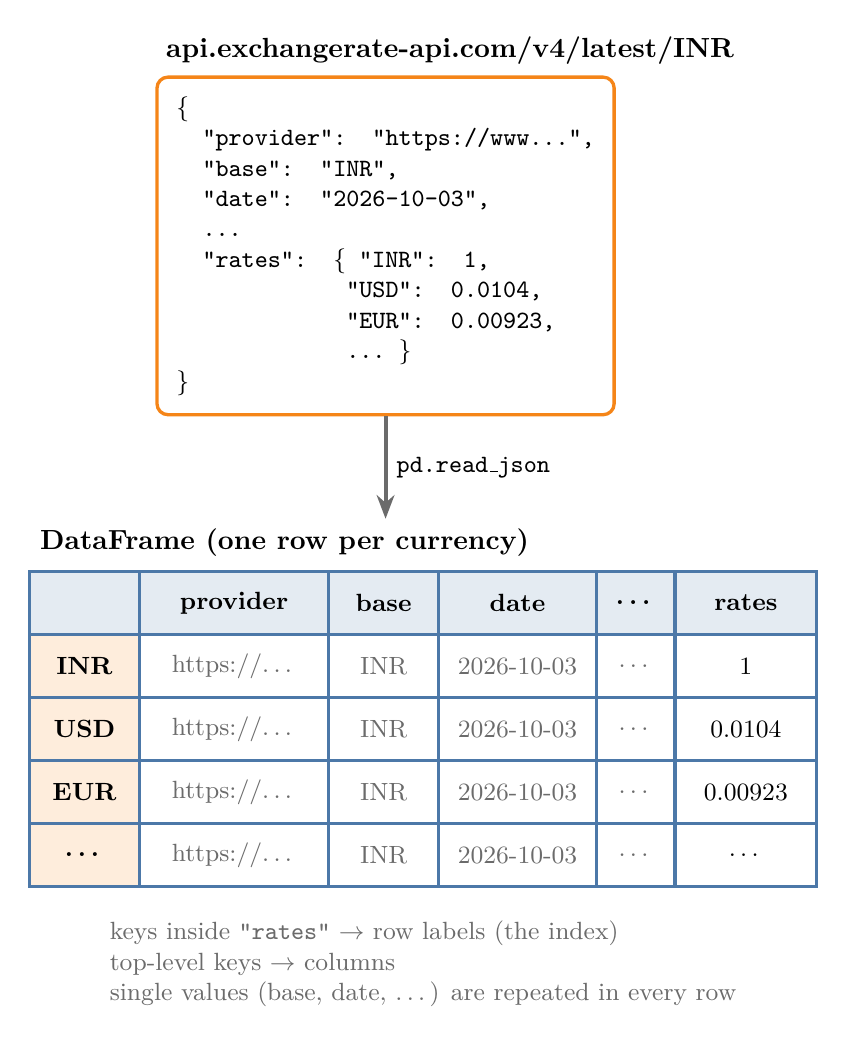
\begin{tikzpicture}
  \node[box=corange, fill=white, align=left, font=\ttfamily\small, anchor=north west] (j) at (0,0) {%
\{\\
\ \ "provider": "https://www...",\\
\ \ "base": "INR",\\
\ \ "date": "2026-10-03",\\
\ \ ...\\
\ \ "rates": \{\ "INR": 1,\\
\ \ \ \ \ \ \ \ \ \ \ \ \ "USD": 0.0104,\\
\ \ \ \ \ \ \ \ \ \ \ \ \ "EUR": 0.00923,\\
\ \ \ \ \ \ \ \ \ \ \ \ \ ...\ \}\\
\}};
  \node[anchor=south west, font=\sffamily\bfseries] at (j.north west) {api.exchangerate-api.com/v4/latest/INR};
  \begin{scope}[shift={(-1.6,-6.7)}, cell/.style={draw=cblue, minimum height=0.8cm, font=\small, inner sep=2pt}]
    \foreach \x/\w/\t in {0.7/1.4/{}, 2.6/2.4/provider, 4.5/1.4/base, 6.2/2.0/date, 7.7/1.0/{\dots}, 9.1/1.8/rates}
      \node[cell, fill=cblue!15, font=\small\bfseries, minimum width=\w cm] at (\x,0) {\t};
    \foreach \y/\c/\r in {-0.8/INR/1, -1.6/USD/0.0104, -2.4/EUR/0.00923, -3.2/{\dots}/{\dots}} {
      \node[cell, fill=corange!15, font=\small\bfseries, minimum width=1.4cm] at (0.7,\y) {\c};
      \node[cell, minimum width=2.4cm, text=cgrey] at (2.6,\y) {https://\dots};
      \node[cell, minimum width=1.4cm, text=cgrey] at (4.5,\y) {INR};
      \node[cell, minimum width=2.0cm, text=cgrey] at (6.2,\y) {2026-10-03};
      \node[cell, minimum width=1.0cm, text=cgrey] at (7.7,\y) {\dots};
      \node[cell, minimum width=1.8cm] at (9.1,\y) {\r};
    }
    \node[anchor=south west, font=\sffamily\bfseries] at (0,0.45) {DataFrame (one row per currency)};
    \node[note, anchor=north, align=left] at (5,-3.9) {keys inside \texttt{"rates"} $\rightarrow$ row labels (the index)\\top-level keys $\rightarrow$ columns\\single values (base, date, \dots) are repeated in every row};
  \end{scope}
  \draw[arrow] (j.south) -- node[right, font=\ttfamily\small]{pd.read\_json} ++(0,-1.3);
\end{tikzpicture}
\end{document}
